Σε αυτή την ενότητα παρουσιάζεται η μεθοδολογία και τα εσωτερικά αποτελέσματα
του PGL-FMIC με ένα παράδειγμα: έστω ο χάρτης που απεικονίζεται στο σχήμα
\ref{fig:02_02_05:corridor_motivation}, και έστω $\bm{x}_a(11.56, 12.20, 0.0)$
[m, m, rad] η πραγματική στάση του ρομπότ. Έστω επίσης μια υπόθεση στάσης
$\bm{x}_c (7.56, 11.20, \pi/4)$ [m, m, rad] μετασχηματισμένη κατά $(-4.0, -1.0,
\pi/4)$ σε σχέση με την πραγματική στάση. Στο στάδιο της εκτίμησης της
περιστροφής του ρομπότ, η μέτρηση που λαμβάνεται από την πραγματική στάση του
ρομπότ, $\mathcal{S}_R^a$, και η εικονική σάρωση που λαμβάνεται από την
υπόθεση, $\mathcal{S}_V^c$, προβάλλονται στο επίπεδο $x-y$ σαν η κάθεμία να
είχε καταγραφεί από τη στάση $Ο(0,0,0)$. Το σχήμα
\ref{fig:pgl_fmic_illustration}(α') δείχνει την προβολή των τελικών σημείων
$\mathcal{P}_R^a$ των ακτίνων του $\mathcal{S}_R^a$, ενώ το σχήμα
\ref{fig:pgl_fmic_illustration}(β') δείχνει εκείνα του $\mathcal{S}_V^c$,
$\mathcal{P}_v^c$.  Παρατηρήστε ότι αυτά τα σύνολα συνδεδεμένων σημείων
αποτελούνται από το περιβάλλον των πραγματικών και εικονικών αισθητήρων σάρωσης
από την προοπτική του τοπικού συστήματος αναφοράς τους. Αυτά τα σύνολα σημείων
μετατρέπονται στη συνέχεια σε δισδιάστατα πλέγματα μέσω διακριτοποίησης,
εισάγονται στον FMI-SPOMF, και η γωνία περιστροφής μεταξύ τους
χρησιμοποιείται για την ευθυγράμμιση του προσανατολισμού της στάσης $\bm{x}_c$
σε σχέση με αυτήν του $\bm{x}_a$.

Αφού διορθωθεί ο προσανατολισμός της υπόθεσης, καταγράφεται μια νέα σάρωση
χάρτη από την ανανεωμένη υπόθεση $\bm{x}_c^\prime$. Στη συνέχεια υπολογίζονται
τα κεντροειδή του συνόλου $\mathcal{P}_R^a$ και του συνόλου σημείων της νέας,
προβεβλημμένης στο δισδιάστατο επίπεδο, σάρωσης χάρτη
$\mathcal{P}_V^{c\prime}$. Το σχήμα \ref{fig:pgl_fmic_illustration}(γ')
απεικονίζει τα συνδεδεμένα σημεία $\mathcal{P}_R^a$ και το κεντροειδές του
πολυγώνου που σχηματίζεται από αυτά $\bm{C}_a(-3.57, -0.78)$ [m, m]. Το σχήμα
\ref{fig:pgl_fmic_illustration}(δ') απεικονίζει τα συνδεδεμένα σημεία
$\mathcal{P}_v^{c\prime}$ και το αντίστοιχο κεντροειδές $\bm{C}_c(0.42, 0.09)$
[m, m]. Παρατηρήστε πώς τα δύο σχήματα είναι σχεδόν πανομοιότυπα, αλλά
διαφέρουν ως προς τη θέση τους στο επίπεδο $x-y$.  Παρατηρήστε επίσης την
ασυμφωνία μεταξύ αυτών των δύο συνόλων σημείων στην αριστερά πλευρά: λόγω της
μετατόπισης μεταξύ των θέσεων των $\bm{x}_a$ και $\bm{x}_c^\prime$, μεγαλύτερο
μέρος του χάρτη είναι ορατό από τη δεύτερη στάση, και επομένως η διαφορά μεταξύ
των κεντροειδών των αντίστοιχων συνόλων σημείων τους $\bm{C}_a - \bm{C}_c =
[3.99, 0.87]^\top$ δεν αντιστοιχεί ακριβώς με τη διαφορά θέσης μεταξύ των δύο
στάσεων, η οποία είναι $[4.0, 1.0]^\top$.  Προσθέτοντας, ωστόσο, τη διαφορά
$\bm{C}_a - \bm{C}_c$ στη θέση της στάσης $\bm{x}_c^\prime$, και
επαναλαμβάνοντας την ίδια διαδικασία εκτίμησης της θέσης της $\bm{x}_c^\prime$
κάνει το σύνολο $\mathcal{P}_V^{c\prime}$ να συγκλίνει στο $\mathcal{P}_R^a$,
και επομένως την υπόθεση $\bm{x}_c^{\prime}$ στη $\bm{x}_a$. Το σχήμα
\ref{fig:pgl_fmic_illustration}(ε') δείχνει το τελικό σύνολο σημείων
$\mathcal{P}_V^{c\prime}$, το οποίο επικαλύπτει στο σχήμα
\ref{fig:pgl_fmic_illustration}(στ') (χρωματισμένο με κόκκινο χρώμα) το σύνολο
$\mathcal{P}_R^a$ (με μαύρο χρώμα).


Το σχήμα \ref{fig:pgl_fmic_illustration} απεικονίζει τη διαδικασία ευθυγράμμισης
και τα εσωτερικά βήματα που ακολουθεί ο αλγόριθμος PGL-FMIC ως προς την
εκτίμηση της στάσης του ρομπότ $\bm{x}_a$ από την εκτίμηση $\bm{x}_c$, στις
συνθήκες του περιβάλλοντος που απεικονίζεται στο σχήμα
\ref{fig:02_02_05:corridor_motivation}.


\begin{figure}\centering
    \begin{subfigure}[t]{0.475\linewidth} \centering
        \hspace{0.5cm}
        % GNUPLOT: LaTeX picture with Postscript
\begingroup
  \makeatletter
  \providecommand\color[2][]{%
    \GenericError{(gnuplot) \space\space\space\@spaces}{%
      Package color not loaded in conjunction with
      terminal option `colourtext'%
    }{See the gnuplot documentation for explanation.%
    }{Either use 'blacktext' in gnuplot or load the package
      color.sty in LaTeX.}%
    \renewcommand\color[2][]{}%
  }%
  \providecommand\includegraphics[2][]{%
    \GenericError{(gnuplot) \space\space\space\@spaces}{%
      Package graphicx or graphics not loaded%
    }{See the gnuplot documentation for explanation.%
    }{The gnuplot epslatex terminal needs graphicx.sty or graphics.sty.}%
    \renewcommand\includegraphics[2][]{}%
  }%
  \providecommand\rotatebox[2]{#2}%
  \@ifundefined{ifGPcolor}{%
    \newif\ifGPcolor
    \GPcolorfalse
  }{}%
  \@ifundefined{ifGPblacktext}{%
    \newif\ifGPblacktext
    \GPblacktexttrue
  }{}%
  % define a \g@addto@macro without @ in the name:
  \let\gplgaddtomacro\g@addto@macro
  % define empty templates for all commands taking text:
  \gdef\gplfronttext{}%
  \gdef\gplfronttext{}%
  \makeatother
  \ifGPblacktext
    % no textcolor at all
    \def\colorrgb#1{}%
    \def\colorgray#1{}%
  \else
    % gray or color?
    \ifGPcolor
      \def\colorrgb#1{\color[rgb]{#1}}%
      \def\colorgray#1{\color[gray]{#1}}%
      \expandafter\def\csname LTw\endcsname{\color{white}}%
      \expandafter\def\csname LTb\endcsname{\color{black}}%
      \expandafter\def\csname LTa\endcsname{\color{black}}%
      \expandafter\def\csname LT0\endcsname{\color[rgb]{1,0,0}}%
      \expandafter\def\csname LT1\endcsname{\color[rgb]{0,1,0}}%
      \expandafter\def\csname LT2\endcsname{\color[rgb]{0,0,1}}%
      \expandafter\def\csname LT3\endcsname{\color[rgb]{1,0,1}}%
      \expandafter\def\csname LT4\endcsname{\color[rgb]{0,1,1}}%
      \expandafter\def\csname LT5\endcsname{\color[rgb]{1,1,0}}%
      \expandafter\def\csname LT6\endcsname{\color[rgb]{0,0,0}}%
      \expandafter\def\csname LT7\endcsname{\color[rgb]{1,0.3,0}}%
      \expandafter\def\csname LT8\endcsname{\color[rgb]{0.5,0.5,0.5}}%
    \else
      % gray
      \def\colorrgb#1{\color{black}}%
      \def\colorgray#1{\color[gray]{#1}}%
      \expandafter\def\csname LTw\endcsname{\color{white}}%
      \expandafter\def\csname LTb\endcsname{\color{black}}%
      \expandafter\def\csname LTa\endcsname{\color{black}}%
      \expandafter\def\csname LT0\endcsname{\color{black}}%
      \expandafter\def\csname LT1\endcsname{\color{black}}%
      \expandafter\def\csname LT2\endcsname{\color{black}}%
      \expandafter\def\csname LT3\endcsname{\color{black}}%
      \expandafter\def\csname LT4\endcsname{\color{black}}%
      \expandafter\def\csname LT5\endcsname{\color{black}}%
      \expandafter\def\csname LT6\endcsname{\color{black}}%
      \expandafter\def\csname LT7\endcsname{\color{black}}%
      \expandafter\def\csname LT8\endcsname{\color{black}}%
    \fi
  \fi
    \setlength{\unitlength}{0.0500bp}%
    \ifx\gptboxheight\undefined%
      \newlength{\gptboxheight}%
      \newlength{\gptboxwidth}%
      \newsavebox{\gptboxtext}%
    \fi%
    \setlength{\fboxrule}{0.5pt}%
    \setlength{\fboxsep}{1pt}%
\begin{picture}(2000.00,2000.00)%
    \gplgaddtomacro\gplfronttext{%
      \colorrgb{0.00,0.00,0.00}%
      \put(128,647){\makebox(0,0)[r]{\strut{}$-4.0$}}%
      \colorrgb{0.00,0.00,0.00}%
      \put(128,929){\makebox(0,0)[r]{\strut{}$-2.0$}}%
      \colorrgb{0.00,0.00,0.00}%
      \put(128,1210){\makebox(0,0)[r]{\strut{}$0.0$}}%
      \colorrgb{0.00,0.00,0.00}%
      \put(128,1492){\makebox(0,0)[r]{\strut{}$2.0$}}%
      \colorrgb{0.00,0.00,0.00}%
      \put(401,195){\makebox(0,0){\strut{}$-8.0$}}%
      \colorrgb{0.00,0.00,0.00}%
      \put(964,195){\makebox(0,0){\strut{}$-4.0$}}%
      \colorrgb{0.00,0.00,0.00}%
      \put(1527,195){\makebox(0,0){\strut{}$0.0$}}%
    }%
    \gplgaddtomacro\gplfronttext{%
      \colorrgb{0.00,0.00,0.00}%
      \put(-428,1034){\rotatebox{90}{\makebox(0,0){\strut{}y [m]}}}%
      \colorrgb{0.00,0.00,0.00}%
      \put(1034,-135){\makebox(0,0){\strut{}x [m]}}%
    }%
    \gplfronttext
    \put(0,0){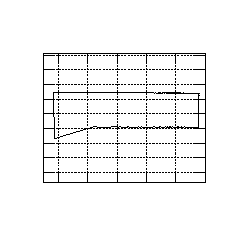
\includegraphics{./figures/parts/appendix/chapters/03/sections/03/real1}}%
    \gplfronttext
  \end{picture}%
\endgroup
\vspace{1em}
        \caption{\small Τα συνδεδεμένα τελικά σημεία $\mathcal{P}_R^a$ της
                 μέτρησης από την πραγματική στάση του ρομπότ $\bm{x}_a$,
                 προβεβλημμένα στο τοπικό σύστημα συντεταγμένων του αισθητήρα}
    \end{subfigure}
    \hfill
    \begin{subfigure}[t]{0.475\linewidth} \centering
        \hspace{0.5cm}
        % GNUPLOT: LaTeX picture with Postscript
\begingroup
  \makeatletter
  \providecommand\color[2][]{%
    \GenericError{(gnuplot) \space\space\space\@spaces}{%
      Package color not loaded in conjunction with
      terminal option `colourtext'%
    }{See the gnuplot documentation for explanation.%
    }{Either use 'blacktext' in gnuplot or load the package
      color.sty in LaTeX.}%
    \renewcommand\color[2][]{}%
  }%
  \providecommand\includegraphics[2][]{%
    \GenericError{(gnuplot) \space\space\space\@spaces}{%
      Package graphicx or graphics not loaded%
    }{See the gnuplot documentation for explanation.%
    }{The gnuplot epslatex terminal needs graphicx.sty or graphics.sty.}%
    \renewcommand\includegraphics[2][]{}%
  }%
  \providecommand\rotatebox[2]{#2}%
  \@ifundefined{ifGPcolor}{%
    \newif\ifGPcolor
    \GPcolorfalse
  }{}%
  \@ifundefined{ifGPblacktext}{%
    \newif\ifGPblacktext
    \GPblacktexttrue
  }{}%
  % define a \g@addto@macro without @ in the name:
  \let\gplgaddtomacro\g@addto@macro
  % define empty templates for all commands taking text:
  \gdef\gplfronttext{}%
  \gdef\gplfronttext{}%
  \makeatother
  \ifGPblacktext
    % no textcolor at all
    \def\colorrgb#1{}%
    \def\colorgray#1{}%
  \else
    % gray or color?
    \ifGPcolor
      \def\colorrgb#1{\color[rgb]{#1}}%
      \def\colorgray#1{\color[gray]{#1}}%
      \expandafter\def\csname LTw\endcsname{\color{white}}%
      \expandafter\def\csname LTb\endcsname{\color{black}}%
      \expandafter\def\csname LTa\endcsname{\color{black}}%
      \expandafter\def\csname LT0\endcsname{\color[rgb]{1,0,0}}%
      \expandafter\def\csname LT1\endcsname{\color[rgb]{0,1,0}}%
      \expandafter\def\csname LT2\endcsname{\color[rgb]{0,0,1}}%
      \expandafter\def\csname LT3\endcsname{\color[rgb]{1,0,1}}%
      \expandafter\def\csname LT4\endcsname{\color[rgb]{0,1,1}}%
      \expandafter\def\csname LT5\endcsname{\color[rgb]{1,1,0}}%
      \expandafter\def\csname LT6\endcsname{\color[rgb]{0,0,0}}%
      \expandafter\def\csname LT7\endcsname{\color[rgb]{1,0.3,0}}%
      \expandafter\def\csname LT8\endcsname{\color[rgb]{0.5,0.5,0.5}}%
    \else
      % gray
      \def\colorrgb#1{\color{black}}%
      \def\colorgray#1{\color[gray]{#1}}%
      \expandafter\def\csname LTw\endcsname{\color{white}}%
      \expandafter\def\csname LTb\endcsname{\color{black}}%
      \expandafter\def\csname LTa\endcsname{\color{black}}%
      \expandafter\def\csname LT0\endcsname{\color{black}}%
      \expandafter\def\csname LT1\endcsname{\color{black}}%
      \expandafter\def\csname LT2\endcsname{\color{black}}%
      \expandafter\def\csname LT3\endcsname{\color{black}}%
      \expandafter\def\csname LT4\endcsname{\color{black}}%
      \expandafter\def\csname LT5\endcsname{\color{black}}%
      \expandafter\def\csname LT6\endcsname{\color{black}}%
      \expandafter\def\csname LT7\endcsname{\color{black}}%
      \expandafter\def\csname LT8\endcsname{\color{black}}%
    \fi
  \fi
    \setlength{\unitlength}{0.0500bp}%
    \ifx\gptboxheight\undefined%
      \newlength{\gptboxheight}%
      \newlength{\gptboxwidth}%
      \newsavebox{\gptboxtext}%
    \fi%
    \setlength{\fboxrule}{0.5pt}%
    \setlength{\fboxsep}{1pt}%
\begin{picture}(2000.00,2000.00)%
    \gplgaddtomacro\gplfronttext{%
      \colorrgb{0.00,0.00,0.00}%
      \put(128,505){\makebox(0,0)[r]{\strut{}$-4.0$}}%
      \colorrgb{0.00,0.00,0.00}%
      \put(128,793){\makebox(0,0)[r]{\strut{}$-2.0$}}%
      \colorrgb{0.00,0.00,0.00}%
      \put(128,1081){\makebox(0,0)[r]{\strut{}$0.0$}}%
      \colorrgb{0.00,0.00,0.00}%
      \put(128,1370){\makebox(0,0)[r]{\strut{}$2.0$}}%
      \colorrgb{0.00,0.00,0.00}%
      \put(431,195){\makebox(0,0){\strut{}$-4.0$}}%
      \colorrgb{0.00,0.00,0.00}%
      \put(1007,195){\makebox(0,0){\strut{}$0.0$}}%
      \colorrgb{0.00,0.00,0.00}%
      \put(1583,195){\makebox(0,0){\strut{}$4.0$}}%
    }%
    \gplgaddtomacro\gplfronttext{%
      \colorrgb{0.00,0.00,0.00}%
      %\put(-378,1034){\rotatebox{90}{\makebox(0,0){\strut{}y [m]}}}%
      \colorrgb{0.00,0.00,0.00}%
      \put(1034,-135){\makebox(0,0){\strut{}x [m]}}%
    }%
    \gplfronttext
    \put(0,0){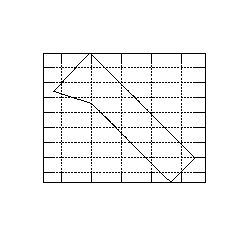
\includegraphics{./figures/parts/appendix/chapters/03/sections/03/virtual1}}%
    \gplfronttext
  \end{picture}%
\endgroup
\vspace{1em}
        \caption{\small Τα συνδεδεμένα τελικά σημεία $\mathcal{P}_V^c$ της
                 εικονικής μέτρησης που συλλαμβάνεται από την υπόθεση στάσης
                 $\bm{x}_c$, προβεβλημμένα στο τοπικό σύστημα συντεταγμένων του
                 εικονικού αισθητήρα}
    \end{subfigure}
    \begin{subfigure}[t]{0.475\linewidth} \centering
        \hspace{0.5cm}
        % GNUPLOT: LaTeX picture with Postscript
\begingroup
  \makeatletter
  \providecommand\color[2][]{%
    \GenericError{(gnuplot) \space\space\space\@spaces}{%
      Package color not loaded in conjunction with
      terminal option `colourtext'%
    }{See the gnuplot documentation for explanation.%
    }{Either use 'blacktext' in gnuplot or load the package
      color.sty in LaTeX.}%
    \renewcommand\color[2][]{}%
  }%
  \providecommand\includegraphics[2][]{%
    \GenericError{(gnuplot) \space\space\space\@spaces}{%
      Package graphicx or graphics not loaded%
    }{See the gnuplot documentation for explanation.%
    }{The gnuplot epslatex terminal needs graphicx.sty or graphics.sty.}%
    \renewcommand\includegraphics[2][]{}%
  }%
  \providecommand\rotatebox[2]{#2}%
  \@ifundefined{ifGPcolor}{%
    \newif\ifGPcolor
    \GPcolorfalse
  }{}%
  \@ifundefined{ifGPblacktext}{%
    \newif\ifGPblacktext
    \GPblacktexttrue
  }{}%
  % define a \g@addto@macro without @ in the name:
  \let\gplgaddtomacro\g@addto@macro
  % define empty templates for all commands taking text:
  \gdef\gplfronttext{}%
  \gdef\gplfronttext{}%
  \makeatother
  \ifGPblacktext
    % no textcolor at all
    \def\colorrgb#1{}%
    \def\colorgray#1{}%
  \else
    % gray or color?
    \ifGPcolor
      \def\colorrgb#1{\color[rgb]{#1}}%
      \def\colorgray#1{\color[gray]{#1}}%
      \expandafter\def\csname LTw\endcsname{\color{white}}%
      \expandafter\def\csname LTb\endcsname{\color{black}}%
      \expandafter\def\csname LTa\endcsname{\color{black}}%
      \expandafter\def\csname LT0\endcsname{\color[rgb]{1,0,0}}%
      \expandafter\def\csname LT1\endcsname{\color[rgb]{0,1,0}}%
      \expandafter\def\csname LT2\endcsname{\color[rgb]{0,0,1}}%
      \expandafter\def\csname LT3\endcsname{\color[rgb]{1,0,1}}%
      \expandafter\def\csname LT4\endcsname{\color[rgb]{0,1,1}}%
      \expandafter\def\csname LT5\endcsname{\color[rgb]{1,1,0}}%
      \expandafter\def\csname LT6\endcsname{\color[rgb]{0,0,0}}%
      \expandafter\def\csname LT7\endcsname{\color[rgb]{1,0.3,0}}%
      \expandafter\def\csname LT8\endcsname{\color[rgb]{0.5,0.5,0.5}}%
    \else
      % gray
      \def\colorrgb#1{\color{black}}%
      \def\colorgray#1{\color[gray]{#1}}%
      \expandafter\def\csname LTw\endcsname{\color{white}}%
      \expandafter\def\csname LTb\endcsname{\color{black}}%
      \expandafter\def\csname LTa\endcsname{\color{black}}%
      \expandafter\def\csname LT0\endcsname{\color{black}}%
      \expandafter\def\csname LT1\endcsname{\color{black}}%
      \expandafter\def\csname LT2\endcsname{\color{black}}%
      \expandafter\def\csname LT3\endcsname{\color{black}}%
      \expandafter\def\csname LT4\endcsname{\color{black}}%
      \expandafter\def\csname LT5\endcsname{\color{black}}%
      \expandafter\def\csname LT6\endcsname{\color{black}}%
      \expandafter\def\csname LT7\endcsname{\color{black}}%
      \expandafter\def\csname LT8\endcsname{\color{black}}%
    \fi
  \fi
    \setlength{\unitlength}{0.0500bp}%
    \ifx\gptboxheight\undefined%
      \newlength{\gptboxheight}%
      \newlength{\gptboxwidth}%
      \newsavebox{\gptboxtext}%
    \fi%
    \setlength{\fboxrule}{0.5pt}%
    \setlength{\fboxsep}{1pt}%
\begin{picture}(2000.00,2000.00)%
    \gplgaddtomacro\gplfronttext{%
      \colorrgb{0.00,0.00,0.00}%
      \put(128,647){\makebox(0,0)[r]{\strut{}$-4.0$}}%
      \colorrgb{0.00,0.00,0.00}%
      \put(128,929){\makebox(0,0)[r]{\strut{}$-2.0$}}%
      \colorrgb{0.00,0.00,0.00}%
      \put(128,1210){\makebox(0,0)[r]{\strut{}$0.0$}}%
      \colorrgb{0.00,0.00,0.00}%
      \put(128,1492){\makebox(0,0)[r]{\strut{}$2.0$}}%
      \colorrgb{0.00,0.00,0.00}%
      \put(401,195){\makebox(0,0){\strut{}$-8.0$}}%
      \colorrgb{0.00,0.00,0.00}%
      \put(964,195){\makebox(0,0){\strut{}$-4.0$}}%
      \colorrgb{0.00,0.00,0.00}%
      \put(1527,195){\makebox(0,0){\strut{}$0.0$}}%
    }%
    \gplgaddtomacro\gplfronttext{%
      \colorrgb{0.00,0.00,0.00}%
      \put(-428,1034){\rotatebox{90}{\makebox(0,0){\strut{}y [m]}}}%
      \colorrgb{0.00,0.00,0.00}%
      \put(1034,-135){\makebox(0,0){\strut{}x [m]}}%
    }%
    \gplfronttext
    \put(0,0){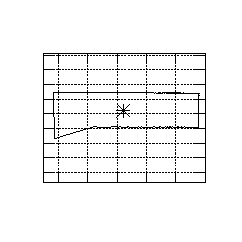
\includegraphics{./figures/parts/appendix/chapters/03/sections/03/real2}}%
    \gplfronttext
  \end{picture}%
\endgroup
\vspace{1em}
        \caption {\small Τα συνδεδεμένα τελικά σημεία $\mathcal{P}_R^a$ της
                 μέτρησης από την πραγματική στάση του ρομπότ $\bm{x}_a$,
                 προβεβλημμένα στο τοπικό σύστημα συντεταγμένων του αισθητήρα,
                 και το κεντροειδές τους}
    \end{subfigure}
    \hfill
    \begin{subfigure}[t]{0.475\linewidth} \centering
        \hspace{0.5cm}
        % GNUPLOT: LaTeX picture with Postscript
\begingroup
  \makeatletter
  \providecommand\color[2][]{%
    \GenericError{(gnuplot) \space\space\space\@spaces}{%
      Package color not loaded in conjunction with
      terminal option `colourtext'%
    }{See the gnuplot documentation for explanation.%
    }{Either use 'blacktext' in gnuplot or load the package
      color.sty in LaTeX.}%
    \renewcommand\color[2][]{}%
  }%
  \providecommand\includegraphics[2][]{%
    \GenericError{(gnuplot) \space\space\space\@spaces}{%
      Package graphicx or graphics not loaded%
    }{See the gnuplot documentation for explanation.%
    }{The gnuplot epslatex terminal needs graphicx.sty or graphics.sty.}%
    \renewcommand\includegraphics[2][]{}%
  }%
  \providecommand\rotatebox[2]{#2}%
  \@ifundefined{ifGPcolor}{%
    \newif\ifGPcolor
    \GPcolorfalse
  }{}%
  \@ifundefined{ifGPblacktext}{%
    \newif\ifGPblacktext
    \GPblacktexttrue
  }{}%
  % define a \g@addto@macro without @ in the name:
  \let\gplgaddtomacro\g@addto@macro
  % define empty templates for all commands taking text:
  \gdef\gplfronttext{}%
  \gdef\gplfronttext{}%
  \makeatother
  \ifGPblacktext
    % no textcolor at all
    \def\colorrgb#1{}%
    \def\colorgray#1{}%
  \else
    % gray or color?
    \ifGPcolor
      \def\colorrgb#1{\color[rgb]{#1}}%
      \def\colorgray#1{\color[gray]{#1}}%
      \expandafter\def\csname LTw\endcsname{\color{white}}%
      \expandafter\def\csname LTb\endcsname{\color{black}}%
      \expandafter\def\csname LTa\endcsname{\color{black}}%
      \expandafter\def\csname LT0\endcsname{\color[rgb]{1,0,0}}%
      \expandafter\def\csname LT1\endcsname{\color[rgb]{0,1,0}}%
      \expandafter\def\csname LT2\endcsname{\color[rgb]{0,0,1}}%
      \expandafter\def\csname LT3\endcsname{\color[rgb]{1,0,1}}%
      \expandafter\def\csname LT4\endcsname{\color[rgb]{0,1,1}}%
      \expandafter\def\csname LT5\endcsname{\color[rgb]{1,1,0}}%
      \expandafter\def\csname LT6\endcsname{\color[rgb]{0,0,0}}%
      \expandafter\def\csname LT7\endcsname{\color[rgb]{1,0.3,0}}%
      \expandafter\def\csname LT8\endcsname{\color[rgb]{0.5,0.5,0.5}}%
    \else
      % gray
      \def\colorrgb#1{\color{black}}%
      \def\colorgray#1{\color[gray]{#1}}%
      \expandafter\def\csname LTw\endcsname{\color{white}}%
      \expandafter\def\csname LTb\endcsname{\color{black}}%
      \expandafter\def\csname LTa\endcsname{\color{black}}%
      \expandafter\def\csname LT0\endcsname{\color{black}}%
      \expandafter\def\csname LT1\endcsname{\color{black}}%
      \expandafter\def\csname LT2\endcsname{\color{black}}%
      \expandafter\def\csname LT3\endcsname{\color{black}}%
      \expandafter\def\csname LT4\endcsname{\color{black}}%
      \expandafter\def\csname LT5\endcsname{\color{black}}%
      \expandafter\def\csname LT6\endcsname{\color{black}}%
      \expandafter\def\csname LT7\endcsname{\color{black}}%
      \expandafter\def\csname LT8\endcsname{\color{black}}%
    \fi
  \fi
    \setlength{\unitlength}{0.0500bp}%
    \ifx\gptboxheight\undefined%
      \newlength{\gptboxheight}%
      \newlength{\gptboxwidth}%
      \newsavebox{\gptboxtext}%
    \fi%
    \setlength{\fboxrule}{0.5pt}%
    \setlength{\fboxsep}{1pt}%
\begin{picture}(2000.00,2000.00)%
    \gplgaddtomacro\gplfronttext{%
      \colorrgb{0.00,0.00,0.00}%
      \put(128,542){\makebox(0,0)[r]{\strut{}$-4.0$}}%
      \colorrgb{0.00,0.00,0.00}%
      \put(128,823){\makebox(0,0)[r]{\strut{}$-2.0$}}%
      \colorrgb{0.00,0.00,0.00}%
      \put(128,1105){\makebox(0,0)[r]{\strut{}$0.0$}}%
      \colorrgb{0.00,0.00,0.00}%
      \put(128,1386){\makebox(0,0)[r]{\strut{}$2.0$}}%
      \colorrgb{0.00,0.00,0.00}%
      \put(401,195){\makebox(0,0){\strut{}$-4.0$}}%
      \colorrgb{0.00,0.00,0.00}%
      \put(964,195){\makebox(0,0){\strut{}$0.0$}}%
      \colorrgb{0.00,0.00,0.00}%
      \put(1527,195){\makebox(0,0){\strut{}$4.0$}}%
    }%
    \gplgaddtomacro\gplfronttext{%
      \colorrgb{0.00,0.00,0.00}%
      %\put(-378,1034){\rotatebox{90}{\makebox(0,0){\strut{}y [m]}}}%
      \colorrgb{0.00,0.00,0.00}%
      \put(1034,-135){\makebox(0,0){\strut{}x [m]}}%
    }%
    \gplfronttext
    \put(0,0){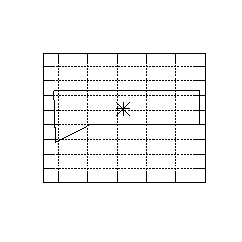
\includegraphics{./figures/parts/appendix/chapters/03/sections/03/virtual2}}%
    \gplfronttext
  \end{picture}%
\endgroup
\vspace{1em}
         \caption{\small Τα συνδεδεμένα τελικά σημεία $\mathcal{P}_V^{c\prime}$
                  της εικονικής μέτρησης που συλλαμβάνεται από τη διορθωμένη
                  κατά προσανατολισμό---αλλά όχι ως προς τη θέση---υπόθεση
                  στάσης $\bm{x}_c^\prime$, προβεβλημμένα στο τοπικό σύστημα
                  συντεταγμένων του εικονικού αισθητήρα, και το κεντροειδές
                  τους. Ας σημειωθεί ότι το πολύγωνο που σχηματίζεται από τα
                  τελικά σημεία έχει ευθυγραμμιστεί ως προς τον προσανατολισμό
                  με το αντίστοιχο πολύγωνο $\mathcal{P}_R^a$, αλλά όχι ως προς
                  τη θέση}
    \end{subfigure}
    \begin{subfigure}[t]{0.475\linewidth} \centering
        \hspace{0.5cm}
        % GNUPLOT: LaTeX picture with Postscript
\begingroup
  \makeatletter
  \providecommand\color[2][]{%
    \GenericError{(gnuplot) \space\space\space\@spaces}{%
      Package color not loaded in conjunction with
      terminal option `colourtext'%
    }{See the gnuplot documentation for explanation.%
    }{Either use 'blacktext' in gnuplot or load the package
      color.sty in LaTeX.}%
    \renewcommand\color[2][]{}%
  }%
  \providecommand\includegraphics[2][]{%
    \GenericError{(gnuplot) \space\space\space\@spaces}{%
      Package graphicx or graphics not loaded%
    }{See the gnuplot documentation for explanation.%
    }{The gnuplot epslatex terminal needs graphicx.sty or graphics.sty.}%
    \renewcommand\includegraphics[2][]{}%
  }%
  \providecommand\rotatebox[2]{#2}%
  \@ifundefined{ifGPcolor}{%
    \newif\ifGPcolor
    \GPcolorfalse
  }{}%
  \@ifundefined{ifGPblacktext}{%
    \newif\ifGPblacktext
    \GPblacktexttrue
  }{}%
  % define a \g@addto@macro without @ in the name:
  \let\gplgaddtomacro\g@addto@macro
  % define empty templates for all commands taking text:
  \gdef\gplfronttext{}%
  \gdef\gplfronttext{}%
  \makeatother
  \ifGPblacktext
    % no textcolor at all
    \def\colorrgb#1{}%
    \def\colorgray#1{}%
  \else
    % gray or color?
    \ifGPcolor
      \def\colorrgb#1{\color[rgb]{#1}}%
      \def\colorgray#1{\color[gray]{#1}}%
      \expandafter\def\csname LTw\endcsname{\color{white}}%
      \expandafter\def\csname LTb\endcsname{\color{black}}%
      \expandafter\def\csname LTa\endcsname{\color{black}}%
      \expandafter\def\csname LT0\endcsname{\color[rgb]{1,0,0}}%
      \expandafter\def\csname LT1\endcsname{\color[rgb]{0,1,0}}%
      \expandafter\def\csname LT2\endcsname{\color[rgb]{0,0,1}}%
      \expandafter\def\csname LT3\endcsname{\color[rgb]{1,0,1}}%
      \expandafter\def\csname LT4\endcsname{\color[rgb]{0,1,1}}%
      \expandafter\def\csname LT5\endcsname{\color[rgb]{1,1,0}}%
      \expandafter\def\csname LT6\endcsname{\color[rgb]{0,0,0}}%
      \expandafter\def\csname LT7\endcsname{\color[rgb]{1,0.3,0}}%
      \expandafter\def\csname LT8\endcsname{\color[rgb]{0.5,0.5,0.5}}%
    \else
      % gray
      \def\colorrgb#1{\color{black}}%
      \def\colorgray#1{\color[gray]{#1}}%
      \expandafter\def\csname LTw\endcsname{\color{white}}%
      \expandafter\def\csname LTb\endcsname{\color{black}}%
      \expandafter\def\csname LTa\endcsname{\color{black}}%
      \expandafter\def\csname LT0\endcsname{\color{black}}%
      \expandafter\def\csname LT1\endcsname{\color{black}}%
      \expandafter\def\csname LT2\endcsname{\color{black}}%
      \expandafter\def\csname LT3\endcsname{\color{black}}%
      \expandafter\def\csname LT4\endcsname{\color{black}}%
      \expandafter\def\csname LT5\endcsname{\color{black}}%
      \expandafter\def\csname LT6\endcsname{\color{black}}%
      \expandafter\def\csname LT7\endcsname{\color{black}}%
      \expandafter\def\csname LT8\endcsname{\color{black}}%
    \fi
  \fi
    \setlength{\unitlength}{0.0500bp}%
    \ifx\gptboxheight\undefined%
      \newlength{\gptboxheight}%
      \newlength{\gptboxwidth}%
      \newsavebox{\gptboxtext}%
    \fi%
    \setlength{\fboxrule}{0.5pt}%
    \setlength{\fboxsep}{1pt}%
\begin{picture}(2000.00,2000.00)%
    \gplgaddtomacro\gplfronttext{%
      \colorrgb{0.00,0.00,0.00}%
      \put(128,647){\makebox(0,0)[r]{\strut{}$-4.0$}}%
      \colorrgb{0.00,0.00,0.00}%
      \put(128,929){\makebox(0,0)[r]{\strut{}$-2.0$}}%
      \colorrgb{0.00,0.00,0.00}%
      \put(128,1210){\makebox(0,0)[r]{\strut{}$0.0$}}%
      \colorrgb{0.00,0.00,0.00}%
      \put(128,1492){\makebox(0,0)[r]{\strut{}$2.0$}}%
      \colorrgb{0.00,0.00,0.00}%
      \put(401,195){\makebox(0,0){\strut{}$-8.0$}}%
      \colorrgb{0.00,0.00,0.00}%
      \put(964,195){\makebox(0,0){\strut{}$-4.0$}}%
      \colorrgb{0.00,0.00,0.00}%
      \put(1527,195){\makebox(0,0){\strut{}$0.0$}}%
      \colorrgb{0.00,0.00,0.00}%
    }%
    \gplgaddtomacro\gplfronttext{%
      \colorrgb{0.00,0.00,0.00}%
      \put(-428,1034){\rotatebox{90}{\makebox(0,0){\strut{}y [m]}}}%
      \colorrgb{0.00,0.00,0.00}%
      \put(1034,-135){\makebox(0,0){\strut{}x [m]}}%
    }%
    \gplfronttext
    \put(0,0){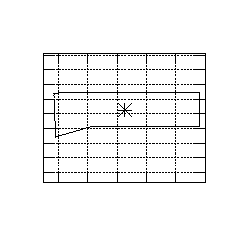
\includegraphics{./figures/parts/appendix/chapters/03/sections/03/virtual3}}%
    \gplfronttext
  \end{picture}%
\endgroup
\vspace{1em}
        \caption{\small Τα συνδεδεμένα τελικά σημεία $\mathcal{P}_V^{c\prime}$ της
                  εικονικής μέτρησης που συλλαμβάνεται από τη διορθωμένη
                  κατά προσανατολισμό και στάση υπόθεση στάσης
                  $\bm{x}_c^\prime$, προβεβλημμένα στο τοπικό σύστημα
                  συντεταγμένων του εικονικού αισθητήρα, και το κεντροειδές
                  τους}
    \end{subfigure}
    \hfill
    \begin{subfigure}[t]{0.475\linewidth} \centering
        \hspace{0.5cm}
        % GNUPLOT: LaTeX picture with Postscript
\begingroup
  \makeatletter
  \providecommand\color[2][]{%
    \GenericError{(gnuplot) \space\space\space\@spaces}{%
      Package color not loaded in conjunction with
      terminal option `colourtext'%
    }{See the gnuplot documentation for explanation.%
    }{Either use 'blacktext' in gnuplot or load the package
      color.sty in LaTeX.}%
    \renewcommand\color[2][]{}%
  }%
  \providecommand\includegraphics[2][]{%
    \GenericError{(gnuplot) \space\space\space\@spaces}{%
      Package graphicx or graphics not loaded%
    }{See the gnuplot documentation for explanation.%
    }{The gnuplot epslatex terminal needs graphicx.sty or graphics.sty.}%
    \renewcommand\includegraphics[2][]{}%
  }%
  \providecommand\rotatebox[2]{#2}%
  \@ifundefined{ifGPcolor}{%
    \newif\ifGPcolor
    \GPcolorfalse
  }{}%
  \@ifundefined{ifGPblacktext}{%
    \newif\ifGPblacktext
    \GPblacktexttrue
  }{}%
  % define a \g@addto@macro without @ in the name:
  \let\gplgaddtomacro\g@addto@macro
  % define empty templates for all commands taking text:
  \gdef\gplfronttext{}%
  \gdef\gplfronttext{}%
  \makeatother
  \ifGPblacktext
    % no textcolor at all
    \def\colorrgb#1{}%
    \def\colorgray#1{}%
  \else
    % gray or color?
    \ifGPcolor
      \def\colorrgb#1{\color[rgb]{#1}}%
      \def\colorgray#1{\color[gray]{#1}}%
      \expandafter\def\csname LTw\endcsname{\color{white}}%
      \expandafter\def\csname LTb\endcsname{\color{black}}%
      \expandafter\def\csname LTa\endcsname{\color{black}}%
      \expandafter\def\csname LT0\endcsname{\color[rgb]{1,0,0}}%
      \expandafter\def\csname LT1\endcsname{\color[rgb]{0,1,0}}%
      \expandafter\def\csname LT2\endcsname{\color[rgb]{0,0,1}}%
      \expandafter\def\csname LT3\endcsname{\color[rgb]{1,0,1}}%
      \expandafter\def\csname LT4\endcsname{\color[rgb]{0,1,1}}%
      \expandafter\def\csname LT5\endcsname{\color[rgb]{1,1,0}}%
      \expandafter\def\csname LT6\endcsname{\color[rgb]{0,0,0}}%
      \expandafter\def\csname LT7\endcsname{\color[rgb]{1,0.3,0}}%
      \expandafter\def\csname LT8\endcsname{\color[rgb]{0.5,0.5,0.5}}%
    \else
      % gray
      \def\colorrgb#1{\color{black}}%
      \def\colorgray#1{\color[gray]{#1}}%
      \expandafter\def\csname LTw\endcsname{\color{white}}%
      \expandafter\def\csname LTb\endcsname{\color{black}}%
      \expandafter\def\csname LTa\endcsname{\color{black}}%
      \expandafter\def\csname LT0\endcsname{\color{black}}%
      \expandafter\def\csname LT1\endcsname{\color{black}}%
      \expandafter\def\csname LT2\endcsname{\color{black}}%
      \expandafter\def\csname LT3\endcsname{\color{black}}%
      \expandafter\def\csname LT4\endcsname{\color{black}}%
      \expandafter\def\csname LT5\endcsname{\color{black}}%
      \expandafter\def\csname LT6\endcsname{\color{black}}%
      \expandafter\def\csname LT7\endcsname{\color{black}}%
      \expandafter\def\csname LT8\endcsname{\color{black}}%
    \fi
  \fi
    \setlength{\unitlength}{0.0500bp}%
    \ifx\gptboxheight\undefined%
      \newlength{\gptboxheight}%
      \newlength{\gptboxwidth}%
      \newsavebox{\gptboxtext}%
    \fi%
    \setlength{\fboxrule}{0.5pt}%
    \setlength{\fboxsep}{1pt}%
\begin{picture}(2000.00,2000.00)%
    \gplgaddtomacro\gplfronttext{%
      \colorrgb{0.00,0.00,0.00}%
      \put(128,647){\makebox(0,0)[r]{\strut{}$-4.0$}}%
      \colorrgb{0.00,0.00,0.00}%
      \put(128,929){\makebox(0,0)[r]{\strut{}$-2.0$}}%
      \colorrgb{0.00,0.00,0.00}%
      \put(128,1210){\makebox(0,0)[r]{\strut{}$0.0$}}%
      \colorrgb{0.00,0.00,0.00}%
      \put(128,1492){\makebox(0,0)[r]{\strut{}$2.0$}}%
      \colorrgb{0.00,0.00,0.00}%
      \put(401,195){\makebox(0,0){\strut{}$-8.0$}}%
      \colorrgb{0.00,0.00,0.00}%
      \put(964,195){\makebox(0,0){\strut{}$-4.0$}}%
      \colorrgb{0.00,0.00,0.00}%
      \put(1527,195){\makebox(0,0){\strut{}$0.0$}}%
    }%
    \gplgaddtomacro\gplfronttext{%
      \colorrgb{0.00,0.00,0.00}%
      %\put(-378,1034){\rotatebox{90}{\makebox(0,0){\strut{}y [m]}}}%
      \colorrgb{0.00,0.00,0.00}%
      \put(1034,-135){\makebox(0,0){\strut{}x [m]}}%
    }%
    \gplfronttext
    \put(0,0){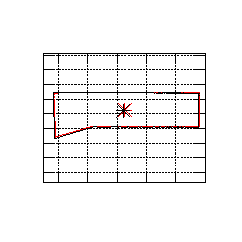
\includegraphics{./figures/parts/appendix/chapters/03/sections/03/aligned}}%
    \gplfronttext
  \end{picture}%
\endgroup
\vspace{1em}
        \caption{\small Τα συνδεδεμένα τελικά σημεία $\mathcal{P}_R^a$ (με
                 μαύρο χρώμα) και $\mathcal{P}_V^{c\prime}$ (κόκκινο), και τα
                 κεντροειδή τους, προβεβλημμένα από τα συστήματα συντεταγμένων
                 των αντίστοιχων αισθητήρων}
    \end{subfigure}
    \caption{\small Η διαδικασία διόρθωσης της υπόθεσης στάσης $\bm{x}_c$
             κατά προσανατολισμό και θέση ως προς την πραγματική στάση του
             ρομπότ $\bm{x}_a$ στο περιβάλλον CORRIDOR (σχήμα
             \ref{fig:02_02_05:corridor_motivation})}
    \label{fig:pgl_fmic_illustration}
\end{figure}

Ας εξετάσουμε τώρα τα πιθανά αποτελέσματα της ίδιας διαδικασίας για μία μη
έγκυρη υποψήφια στάση, έστω την $\bm{x}_b$ του ίδιου σχήματος. Θεωρητικά η
$\bm{x}_b$ είτε θα απορριφθεί στο τέλος της διαδικασίας εκτίμησης
προσανατολισμού λόγω της εξαγωγής ενός αυθαίρετου συντελεστή κλίμακας $\sigma
\in (-\infty, \underline{\sigma}] \cup [\overline{\sigma}, +\infty)$, ή θα
γίνει αποδεκτή για την εκτίμηση της στάσης, οπότε η θέση της υπόθεσης θα
μετακινείτο κατά πάσα πιθανότητα σε πορεία αποκλίνουσα από την πραγματική θέση
του ρομπότ. Εάν $\bm{x}_c \in \mathcal{H}$ τότε ο FMI-SPOMF θα ανέφερε
υψηλότερο βαθμό ομοιότητας $w_c > w_b$, και η υπόθεση $\bm{x}_b$ θα
φιλτραριζόταν ως αληθώς αρνητική υπόθεση. Συνεπώς, εάν καμία υπόθεση στάσης δεν
βρισκόταν στην περιοχή γύρω από τη θέση της στάσης $\bm{x}_a$, η προβαλλόμενες
εικόνες εικονικών μετρήσεων που έχουν ληφθεί από κάθε υπόθεση δεν θα ήταν σε
θέση να ευθυγραμμιστούν από τον FMI-SPOMF, και μια ψευδής υπόθεση θα αναφερόταν
λανθασμένα ως εκτίμηση της στάσης του συστήματος. Αυτό οδηγεί στη διατύπωση της
κάτωθι παρατήρησης:

\begin{remark}
  \label{appendix:remark:02_03_04:hypotheses_number}
  Η ύπαρξη μίας υπόθεσης στάσης $\bm{h} \in \mathcal{H}$ που βρίσκεται στη
  γειτονιά της αληθινής στάσης του ρομπότ είναι αναγκαία συνθήκη για τη σωστή
  λύση του προβλήματος \ref{prob:02_03:the_problem} (με την έννοια της
  παρατήρησης \ref{remark:01_01_02_02:01} υπό το πρίσμα της παραδοχής
  \ref{assumption:02_03_01:02}). Κατά συνέπεια: ο παρεχόμενος αριθμός των
  υποθέσεων στάσης $|\mathcal{H}|$ θα πρέπει να είναι ανάλογος με το εμβαδό
  του χάρτη $\bm{M}$.\footnote{Αυτή η παρατήρηση είναι γενική και υποθέτει ότι καθώς
  αυξάνεται το εμβαδόν ενός περιβάλλοντος , το ίδιο συμβαίνει και με τον ελεύθερό
  του χώρο. Σε απλά περιβάλλοντα, όπως αυτά της δομής του περιβάλλοντος
  CORRIDOR, μπορεί να απαιτούνται λιγότερες υποθέσεις λόγω της μειωμένης
  ύπαρξης δομών που αποκρύπτουν το σύνολο του περιβάλλοντος.}
\end{remark}

Σε πιο σύνθετα περιβάλλοντα, όπου το περιβάλλον και τα χαρακτηριστικά του χάρτη
του εμφανίζουν επαναλαμβανόμενες δομές, μπορεί η ασάφεια στάσης να μην μπορεί
να επιλυθεί, ανεξάρτητα από τον αριθμό των υποθέσεων στάσης. Άλλα περιβάλλοντα,
με μεγάλους ανοιχτούς χώρους, μπορεί να οδηγήσουν σε έλλειψη πληροφοριών λόγω
των ορίων μέγιστης εμβέλειας του αισθητήρα απόστασης. Οι επιπτώσεις αυτών των
συνθηκών μπορεί να είναι τόσο έντονες ώστε να καταγράφεται υψηλότερη ομοιότητα
μεταξύ μιας λανθασμένης στάσης και της πραγματικής στάσης του ρομπότ από ό,τι
μεταξύ της πραγματικής στάσης του ρομπότ και μιας στάσης που βρίσκεται σε μία
γειτονία της. Το πρώτο ζήτημα δυσχεραίνει όλες τις μεθόδους εκτίμησης στάσης
βάσει καθολικής αβεβαιότητας, καθώς, ακόμη και για έναν άνθρωπο, η λύση του
είναι δύσκολη και απαιτεί μέγιστη ευαισθησία διάκρισης διαφορών. Το δεύτερο
ζήτημα είναι επίσης ανεξέλεγκτο, καθώς εκδηλώνεται ως περιορισμός που
επιβάλλεται από τον αυθαίρετο συνδυασμό περιβάλλοντος και εξοπλισμού.
